\chapter{Conclusions and Future Work}
\label{chap:conclusion}
\chaptoc{}

% ########################################

\newpage
\section{Summary and Conclusions}
\label{sec:conclusion}
\begin{colsection}

% ~~~~~~~~~~~~~~~~~~~~

\begin{colsection}

In this thesis I have described my work as part of the GOTO project, primarily working on the control software in order to create a fully-autonomous robotic telescope. After several years of development and commissioning the prototype GOTO telescope is fully operational, and observing from La Palma most nights with no human interaction.

\end{colsection}

% ~~~~~~~~~~~~~~~~~~~~

\subsection{Telescope control}
\label{sec:control_results}
\begin{colsection}

The core of my work has been the \glsfirst{gtecs}, a complete software package split across several Python modules that controls every aspect of the telescope. The hardware control daemons interface with the dome, mount and cameras (see \aref{chap:gtecs}) while the ``pilot'' master control program and its associated systems (see \aref{chap:autonomous}) allow the telescope to function with no human involvement. GOTO has now been operating successfully for months with the pilot in full control. The conditions monitoring systems have proven robust enough to trust the telescope to close in bad weather, and when the occasional unexpected hardware issues do occur the pilot recovery systems can fix the problem and resume observing in a majority of cases before a human even has time to log in. Of course commissioning was not entirely without incident, as described in \aref{chap:commissioning}. However all the software challenges were overcome, and the majority of the delays to GOTO were due to hardware faults which were out of my purview.

Each set of exposures taken with the G-TeCS camera daemon are assigned an incremental run number. From the initial installation in the summer of 2017 up until September 2019 GOTO has taken over 185,000 such exposure sets, and produced many tens of terabytes of data. My role ends when each image has been saved to a file, whereupon they are copied to the master archive in Warwick and backups at other partner institutions.

\end{colsection}

% ~~~~~~~~~~~~~~~~~~~~
\newpage
\subsection{Scheduling and alert follow-up}
\label{sec:gw_results}
\begin{colsection}

GOTO needed a observation scheduling system that could deal with both the survey and follow-up modes. The scheduler used by G-TeCS is a just-in-time system, where the highest priority target is recalculated every time the scheduler is called. This makes it very reactive to transient alerts, which was a requirement of the project. As described above the scheduler has been operating as parted of the automated systems for several months, and GOTO has been reliably taking regular observations.

From the beginning of the LIGO-Virgo third observing run (O3) in April 2019 up until the end of August the LVC released 32 alerts. The G-TeCS sentinel received and reacted to every one of these events, with the results given in \aref{tab:obs_log}. In a few cases the event handler initially failed to process the VOEvent or the skymap, and required manual intervention. As described in
\aref{sec:challenges}
this was usually due to a problem in the LIGO GraceDB, and changes to the GOTO-alert code were made to work around the problem in the future. Each event had pointings added to the observation database, and observations were taken for 25 of the 32 events, of which three were later retracted. Of the remaining seven cases four alerts were received during the day on La Palma and were then retracted before sunset. Only three of the 25 real events had no part of the skymap visible from La Palma.

For events that occurred during the night on La Palma the GOTO-alert event handling system allowed the pilot to immediately begin observations of the visible skymap. As shown in \aref{tab:obs_log} this was the case for eight of the 32 alerts, and in all but one case the first exposure was started less than 60 seconds after the sentinel received the notice. The time delay varies between 30 and 56 seconds, this range will depend on how far the mount had to slew from its previous target. A significant amount of the remaining delay due to having to download the large LVC skymaps from GraceDB, with the rest due to various small delays in the sentinel and pilot, such as the pilot needing to wait for the next scheduler check. Future optimisation might be possible to reduce these delays further. The one exception to this pattern was event S190513bm, which was immediately visible but observations were delayed by 4 minutes. In this case the observations could have started earlier, but at the time the alert was received the pilot was already observing a pointing from the S190512at event received the previous day. As both events were black hole binaries they were inserted at the same rank, and as detailed in
\aref{sec:event_strategy}
equal-rank ToO pointings won't interrupt each other, so the new pointing had to wait until the previous one was completed. In all other cases the pilot was observing a lower-rank target, usually a survey tile, which was immediately aborted when the scheduler check returned the ToO gravitational wave pointing.

\begin{sidewaystable}[p]
    \begin{footnotesize}
    \begin{center}
        \begin{tabular}{l|cccrl} % chktex 44

            \multicolumn{1}{c|}{Event} &
            Event time &
            Alert received &
            Observation start &
            \multicolumn{1}{c}{$\Delta T$ (h)} &
            Notes
            \\
            \midrule
            \textcolor{Red}{S190405ar} &
            2019--04--05 16:01:30 &
            2019--04--12 15:07:26 &
            --- &
            --- &
            \textit{(Retracted before sunset)}
            \\
            S190408an &
            2019--04--08 18:18:02 &
            2019--04--08 19:02:50 &
            2019--04--09 05:40:39 &
            10.63 &

            \\
            S190412m &
            2019--04--12 05:30:44 &
            2019--04--12 06:31:39 &
            2019--04--12 20:28:35 &
            13.95 &
            See GCN \citet{GW190412_GOTO}
            \\
            S190421ar &
            2019--04--21 21:38:56 &
            2019--04--22 16:26:24 &
            2019--04--23 21:54:59 &
            29.48 &

            \\
            S190425z &
            2019--04--25 08:18:05 &
            2019--04--25 09:00:56 &
            2019--04--25 20:38:22 &
            11.62 &
            See GCN \citet{GW190425_GOTO}
            \\
            S190426c &
            2019--04--26 15:21:55 &
            2019--04--26 15:47:11 &
            2019--04--26 20:38:45 &
            4.86 &
            See GCN \citet{GW190426_GOTO}
            \\
            S190503bf &
            2019--05--03 18:54:04 &
            2019--05--03 19:30:15 &
            --- &
            --- &
            \textit{(Never visible from La Palma)}
            \\
            S190510g &
            2019--05--10 02:59:39 &
            2019--05--10 04:21:59 &
            2019--05--10 04:22:55 &
            0.02 &
            Observations began \textbf{56\,s} after notice received
            \\
            S190512at &
            2019--05--12 18:07:14 &
            2019--05--12 18:59:01 &
            2019--05--12 20:53:20 &
            1.91 &

            \\
            S190513bm &
            2019--05--13 20:54:28 &
            2019--05--13 21:21:51 &
            2019--05--13 21:26:19 &
            0.07 &
            Observations began \textbf{4\,min} after notice received
            \\
            S190517h &
            2019--05--17 05:51:01 &
            2019--05--17 06:26:48 &
            2019--05--17 21:42:06 &
            15.26 &

            \\
            \textcolor{Red}{S190518bb} &
            2019--05--18 19:19:19 &
            2019--05--18 19:25:49 &
            --- &
            --- &
            \textit{(Retracted before sunset)}
            \\
            S190519bj &
            2019--05--19 15:35:44 &
            2019--05--19 17:01:40 &
            2019--05--19 20:55:19 &
            3.89 &

            \\
            S190521g &
            2019--05--21 03:02:29 &
            2019--05--21 03:08:49 &
            2019--05--21 03:09:17 &
            0.01 &
            Observations began \textbf{28\,s} after notice received
            \\
            S190521r &
            2019--05--21 07:43:59 &
            2019--05--21 07:50:27 &
            2019--05--21 22:54:03 &
            15.06 &

            \\
            \textcolor{Red}{S190524q} &
            2019--05--24 04:52:06 &
            2019--05--24 04:58:40 &
            2019--05--24 04:59:33 &
            0.01 &
            Observations began \textbf{53\,s} after notice received
            \\
            S190602aq &
            2019--06--02 17:59:27 &
            2019--06--02 18:06:01 &
            --- &
            --- &
            \textit{(Never visible from La Palma)}
            \\
            S190630ag &
            2019--06--30 18:52:05 &
            2019--06--30 18:55:47 &
            2019--06--30 21:14:49 &
            2.32 &

            \\
            S190701ah &
            2019--07--01 20:33:06 &
            2019--07--01 20:38:06 &
            --- &
            --- &
            \textit{(Never visible from La Palma)}
            \\
            S190706ai &
            2019--07--06 22:26:41 &
            2019--07--06 22:44:31 &
            2019--07--06 22:45:09 &
            0.01 &
            Observations began \textbf{38\,s} after notice received
            \\
            S190707q &
            2019--07--07 09:33:26 &
            2019--07--07 10:13:24 &
            2019--07--07 21:54:47 &
            11.69 &

            \\
            S190718y &
            2019--07--18 14:35:12 &
            2019--07--18 15:03:13 &
            2019--07--18 21:08:53 &
            6.09 &

            \\
            S190720a &
            2019--07--20 00:08:36 &
            2019--07--20 00:11:26 &
            2019--07--20 00:11:57 &
            0.01 &
            Observations began \textbf{31\,s} after notice received
            \\
            S190727h &
            2019--07--27 06:03:33 &
            2019--07--27 06:12:02 &
            2019--07--27 21:03:40 &
            14.86 &

            \\
            S190728q &
            2019--07--28 06:45:10 &
            2019--07--28 06:59:32 &
            2019--07--28 21:29:58 &
            14.51 &

            \\
            \textcolor{Red}{S190808ae} &
            2019--08--08 22:21:21 &
            2019--08--08 22:28:00 &
            2019--08--08 22:28:31 &
            0.01 &
            Observations began \textbf{31\,s} after notice received
            \\
            S190814bv &
            2019--08--14 21:10:39 &
            2019--08--14 21:31:44 &
            2019--08--14 22:59:27 &
            1.46 &
            See GCN \citet{GW190814_GOTO}
            \\
            \textcolor{Red}{S190816i} &
            2019--08--16 13:04:31 &
            2019--08--16 13:11:35 &
            --- &
            --- &
            \textit{(Retracted before sunset)}
            \\
            \textcolor{Red}{S190822c} &
            2019--08--22 01:29:59 &
            2019--08--22 01:37:00 &
            2019--08--22 01:37:30 &
            0.01 &
            Observations began \textbf{30\,s} after notice received
            \\
            S190828j &
            2019--08--28 06:34:05 &
            2019--08--28 06:50:14 &
            2019--08--28 22:38:25 &
            15.80 &

            \\
            S190828l &
            2019--08--28 06:55:09 &
            2019--08--28 07:17:46 &
            2019--08--28 23:48:38 &
            16.51 &

            \\
            \textcolor{Red}{S190829u} &
            2019--08--29 21:05:56 &
            2019--08--29 21:17:14 &
            --- &
            --- &
            \textit{(Retracted before sunset)}
            \\

        \end{tabular}
    \end{center}
    \end{footnotesize}
    \caption[GOTO observation log for O3 events so far]{
        GOTO observation log for O3 events up to the end of August 2019. \textcolorbf{Red}{Red} events were later retracted.
    }\label{tab:obs_log}
\end{sidewaystable}

As described back in \aref{sec:gw_detections}, three of the 25 real events detected in O3 so far were the most likely to have a potential electromagnetic counterpart: S190425z, S190426c and S190814bv were all classified as originating from either a binary neutron star or neutron star-black hole binary. These were the most important events to follow up, and the GOTO response to each was reported in the GCN notices \citet{GW190425_GOTO, GW190426_GOTO, GW190814_GOTO}. After analysis no counterparts were found for either of the three events, by GOTO or other projects. The S190814bv skymap had a 90\% contour covering only 23 square degrees, which made it very easy to cover with GOTO;\@ on the other hand the initial skymaps for S190425z and S190426c covered areas of 10,000 sq deg and 1,900 sq deg respectively. The follow-up of both was also complicated by having two viable events occurring within 36 hours of each other. Ultimately in the first two days after the alerts GOTO covered 30\% of the S190425z probability \citep{GW190425_GOTO} and 54\% of the S190426c probability \citep{GW190426_GOTO}, and the coverage maps are shown in \aref{fig:190425_goto} and \aref{fig:190426_goto}.

For these events the follow-up code has been shown to be fast and reliable. Based on this performance if, or when, another GW170817-like event is detected GOTO should be ready and observing the counterpart within 60 seconds of the alert being received.

\begin{figure}[p]
    \begin{center}
        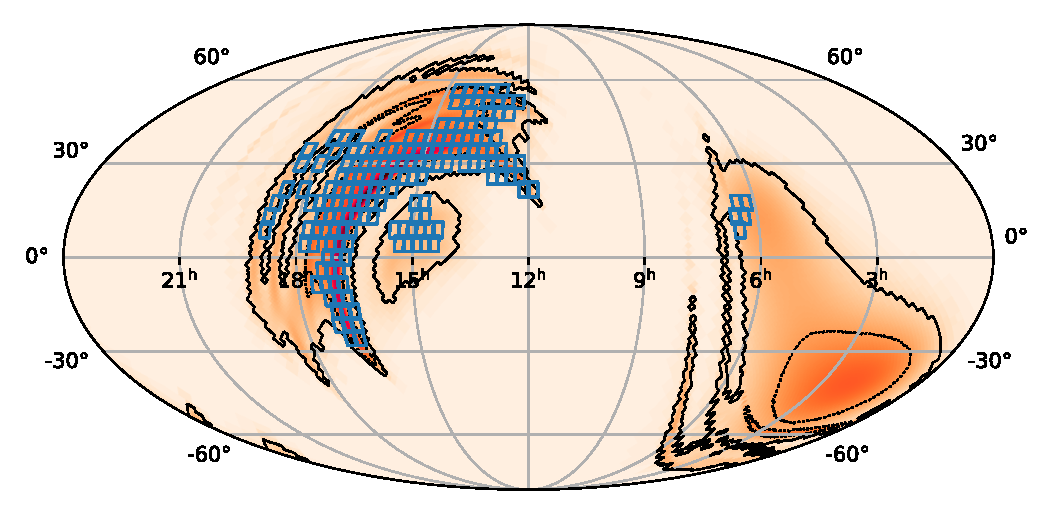
\includegraphics[width=0.9\linewidth]{images/190425_goto.pdf}
    \end{center}
    \caption[Follow-up observations of S190425z with GOTO]{
        Follow-up observations of S190425z with GOTO.\@ The tiled observations are shown in \textcolorbf{NavyBlue}{blue}, over the background BAYESTAR skymap in \textcolorbf{Orange}{orange}. Compare to \aref{fig:ztf} showing ZTF's coverage of the same event.
        }\label{fig:190425_goto}
\end{figure}

\begin{figure}[p]
    \begin{center}
        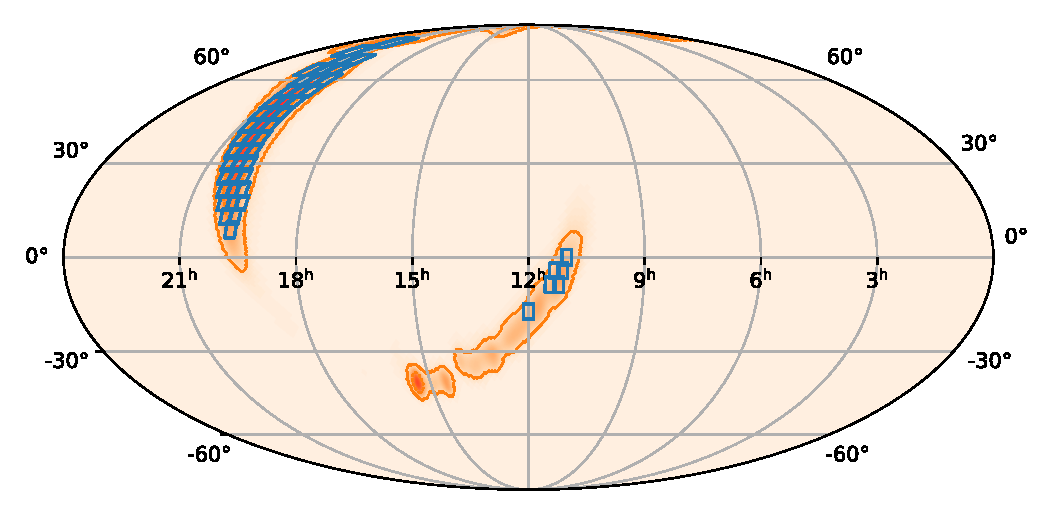
\includegraphics[width=0.9\linewidth]{images/190426_goto.pdf}
    \end{center}
    \caption[Follow-up observations of S190426c with GOTO]{
        Follow-up observations of S190426c with GOTO.\@ The tiled observations are shown in \textcolorbf{NavyBlue}{blue}, over the background BAYESTAR skymap in \textcolorbf{Orange}{orange}.
        }\label{fig:190426_goto}
\end{figure}

\clearpage

\end{colsection}

% ~~~~~~~~~~~~~~~~~~~~

\end{colsection}

% ########################################

\newpage
\section{Future work}
\label{sec:future}
\begin{colsection}

% ~~~~~~~~~~~~~~~~~~~~

\begin{colsection}

This thesis only details the beginning of the GOTO project, and the work described will need to be continued and built upon as the project expands in the future.

\end{colsection}

% ~~~~~~~~~~~~~~~~~~~~

\subsection{The global control system}
\label{sec:gtecs_future}
\begin{colsection}

The obvious direction of future work will be adapting and expanding G-TeCS in order to match the expansion of GOTO.\@

% ---------
\subsubsection{Stage 2}

The next stage, adding the second set of 4 unit telescopes to the existing mount, should require nothing more than a few configuration changes to handle the new \code{fli} interface daemons. On the scheduling side the observation database will need to be reset to handle the new all-sky grid, based on the GOTO-8 field of view instead of the existing GOTO-4 grid. With the change of grid some of the observing strategy detailed in
\aref{chap:alerts}
could be revisited; in particular since each tile will cover a larger area the tile selection algorithm described in
\aref{sec:mapping_skymaps}
might need to be adjusted. Aside from this nothing else should require major changes, and the current pilot will be able to resume observations immediately.

% ---------
\subsubsection{Stage 3}

The addition of the second mount on La Palma will require more control system development. With two telescopes of the same design it would be simple to copy-and-paste the control system and have them operate completely independently. Some systems could be shared between the two domes, and a proposed system diagram is shown in \aref{fig:flow2}.  For example, there would be no need to have two conditions daemons both monitoring the same site masts. But, as described in
\aref{sec:multi_tel_scheduling},
the great benefit of having two telescopes is having them share a common scheduling system. This could be as simple as the system adopted for the multi-telescope simulations in that section, marking one telescope as the primary that always observes the highest-priority pointing and having the other always observe the second-highest. But in reality the telescopes will never be perfectly in sync, and there are more benefits to be gained from a more advanced scheduling system.

\begin{figure}[t]
    \begin{center}
        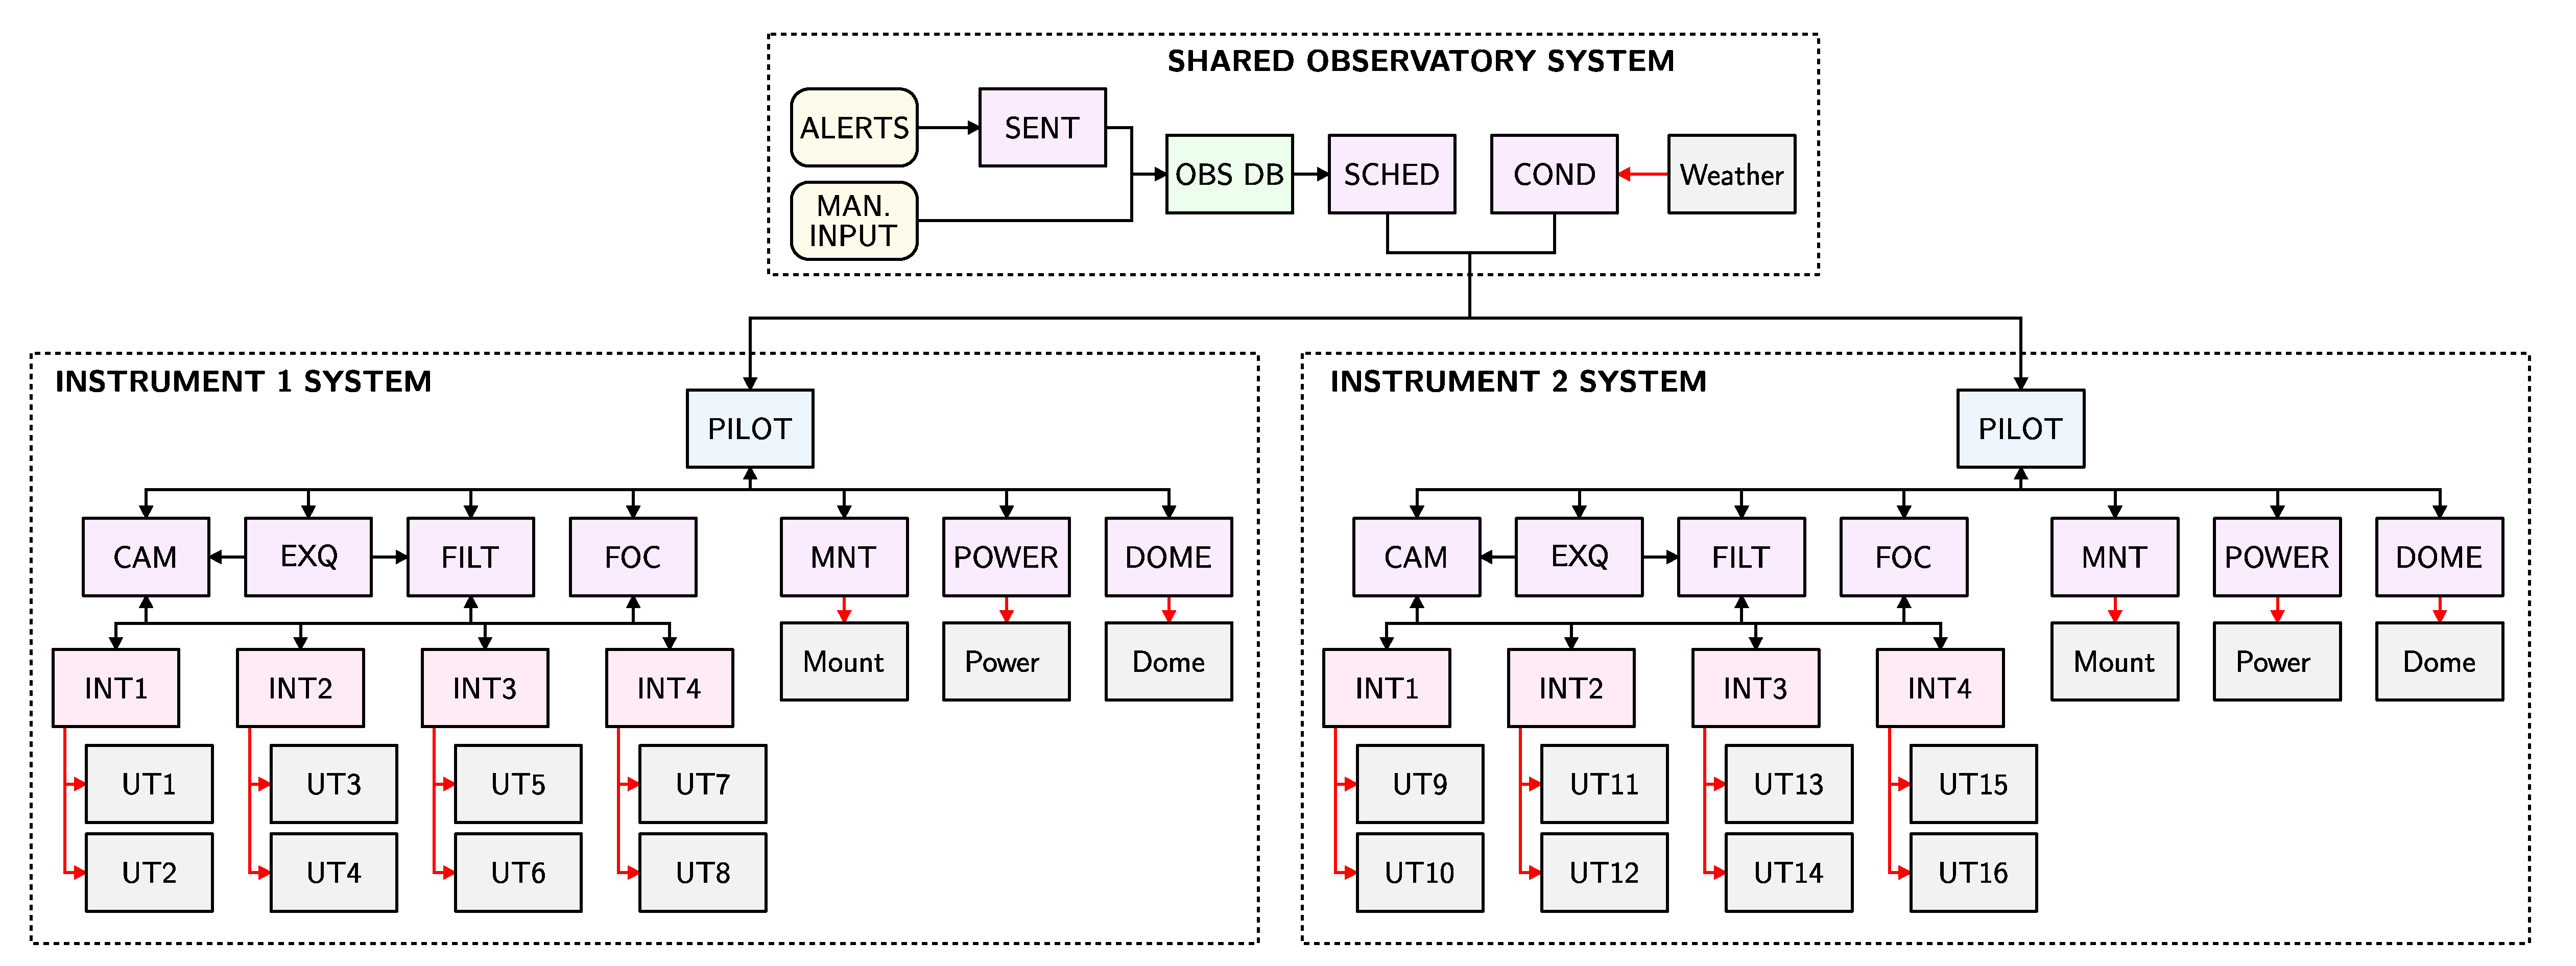
\includegraphics[width=\linewidth]{images/flow2.pdf}
    \end{center}
    \caption[Future G-TeCS system architecture for two telescopes]{
        Proposed future system architecture G-TeCS controlling two telescopes on the same site. Note the two pilots share the same scheduler and conditions daemons but are otherwise independent.
    }\label{fig:flow2}
\end{figure}

Just as the current scheduler described in
\aref{chap:scheduling}
has to decide what to observe based on various constraints, the next-generation scheduler will need to optimise which target is being observed by each telescope. Although several of the constraints will be the same for both mounts (e.g.\ the Moon phase or Sun altitude) it is possible that the two telescopes could have different horizons and therefore altitude limits. The scheduler tie-breaking system will need to be revisited to account for distributing pointings to either telescope. One possible parameter to add to decide which telescope to send a pointing to would be the distance each mount would need to slew from the current target, and a particularly advanced system might also want to account for the time left on the current observations (e.g.\ telescope 1 might be ready to observe while telescope 2 has 10 seconds left on the current target; if the difference in slew times to the new pointing is greater than \SI{10}{\second} then it would be better to wait for telescope 2 to finish).

The move from one 8-UT mount to two 8-UT mounts should mean the same grid can be used, as long as both have the same field of view (see
\aref{sec:multi_grid_scheduling}
for the problems inherent in observing with multiple different grids). However multiple telescopes opens up opportunities for many more advanced observing strategies. They could both observe different parts of the sky to cover the survey or alert skymaps quicker, or they could observe the same point to achieve a greater depth when the images are stacked. The simulations in
\aref{chap:multiscope}
assumed the former in all cases to get the fastest possible coverage, however ideally the future scheduling system should be designed to allow these coordinated observations if required. The presence of the coloured filters adds even more possibilities and complexity. It should be possible to have the two telescopes observe the same target simultaneously but using different filters, to get immediate colour information on any sources. It might also be desired to accept the hit to survey cadence but have each telescope carry out an independent survey in different filters, or perhaps have one taking rapid \SI{60}{\second} exposures while the other takes longer takes longer but uses a meridian scanning method as detailed in
\aref{survey_sim_meridian}.
The possibilities will be huge, and although the ultimate decision will be made depending on the science needs of the GOTO collaboration ideally the scheduling system will be able to handle whatever strategy is desired.

% ---------
\subsubsection{Stage 4}

The final form of the GOTO project is intended to include multiple telescopes at different sites across the globe. This is unlikely to happen before the second mount is built on La Palma, so by the time an Australian site is added the advanced systems described above should already be in place and ideally the next-generation scheduler should be able to delegate observations to multiple telescopes wherever they are in the world. There are several existing projects that operate in this manner which GOTO can emulate, such as the \glsfirst{lco} network \citep{LCO_scheduling}.

\end{colsection}

% ~~~~~~~~~~~~~~~~~~~~
\newpage
\subsection{Continued development}
\label{sec:software_future}
\begin{colsection}

The work described in the previous section will be important to carry out as GOTO expands, however it will also naturally be directed by the timeline of the project going forwards. In general there is still plenty of software development work to do that is less dependent on the GOTO funding situation.

One particular future area of importance should be better integration between the control system and the later analysis pipeline and candidate marshal described in
\aref{sec:gotophoto}.
To achieve a fully autonomous system the pipeline should be able to reschedule observations independently, for example if an image is affected by clouds. More excitingly a future detection algorithm might be permitted to automatically schedule follow-up observations of promising candidates.

Another future direction that is being considered is the generalisation of some or all of the G-TeCS code, removing the GOTO-specific parts and making it usable by other projects. For example, the GOTO-tile code for creating survey grids and mapping skymaps to them described in
\aref{chap:tiling}
is not at all GOTO-specific, and would only require a small amount to work to rewrite into a separate Astropy-compatible Python module (probably along with a new name). On a wider scale the G-TeCS control system could be adapted for other telescopes, and a parallel version is already being used by the other Warwick telescopes on La Palma.

Overall the GOTO Telescope Control System is still under active development, which will continue as the GOTO project evolves. Based on the initial results from O3 the system has been working well and fulfilling its requirements, and it is therefore only a matter of time until GOTO observes the next gravitational wave counterpart.

\end{colsection}

% ~~~~~~~~~~~~~~~~~~~~

\end{colsection}

% ########################################
